\documentclass{article}
\usepackage{amsmath}
\usepackage{amsfonts}
\usepackage{amssymb}
\usepackage{cancel}

\usepackage{graphicx}


\setlength\parindent{0pt}

\author{Pranav Tikkawar}
\title{TODO}

\begin{document}
\maketitle
\section*{Question 1}
\subsection*{a)}
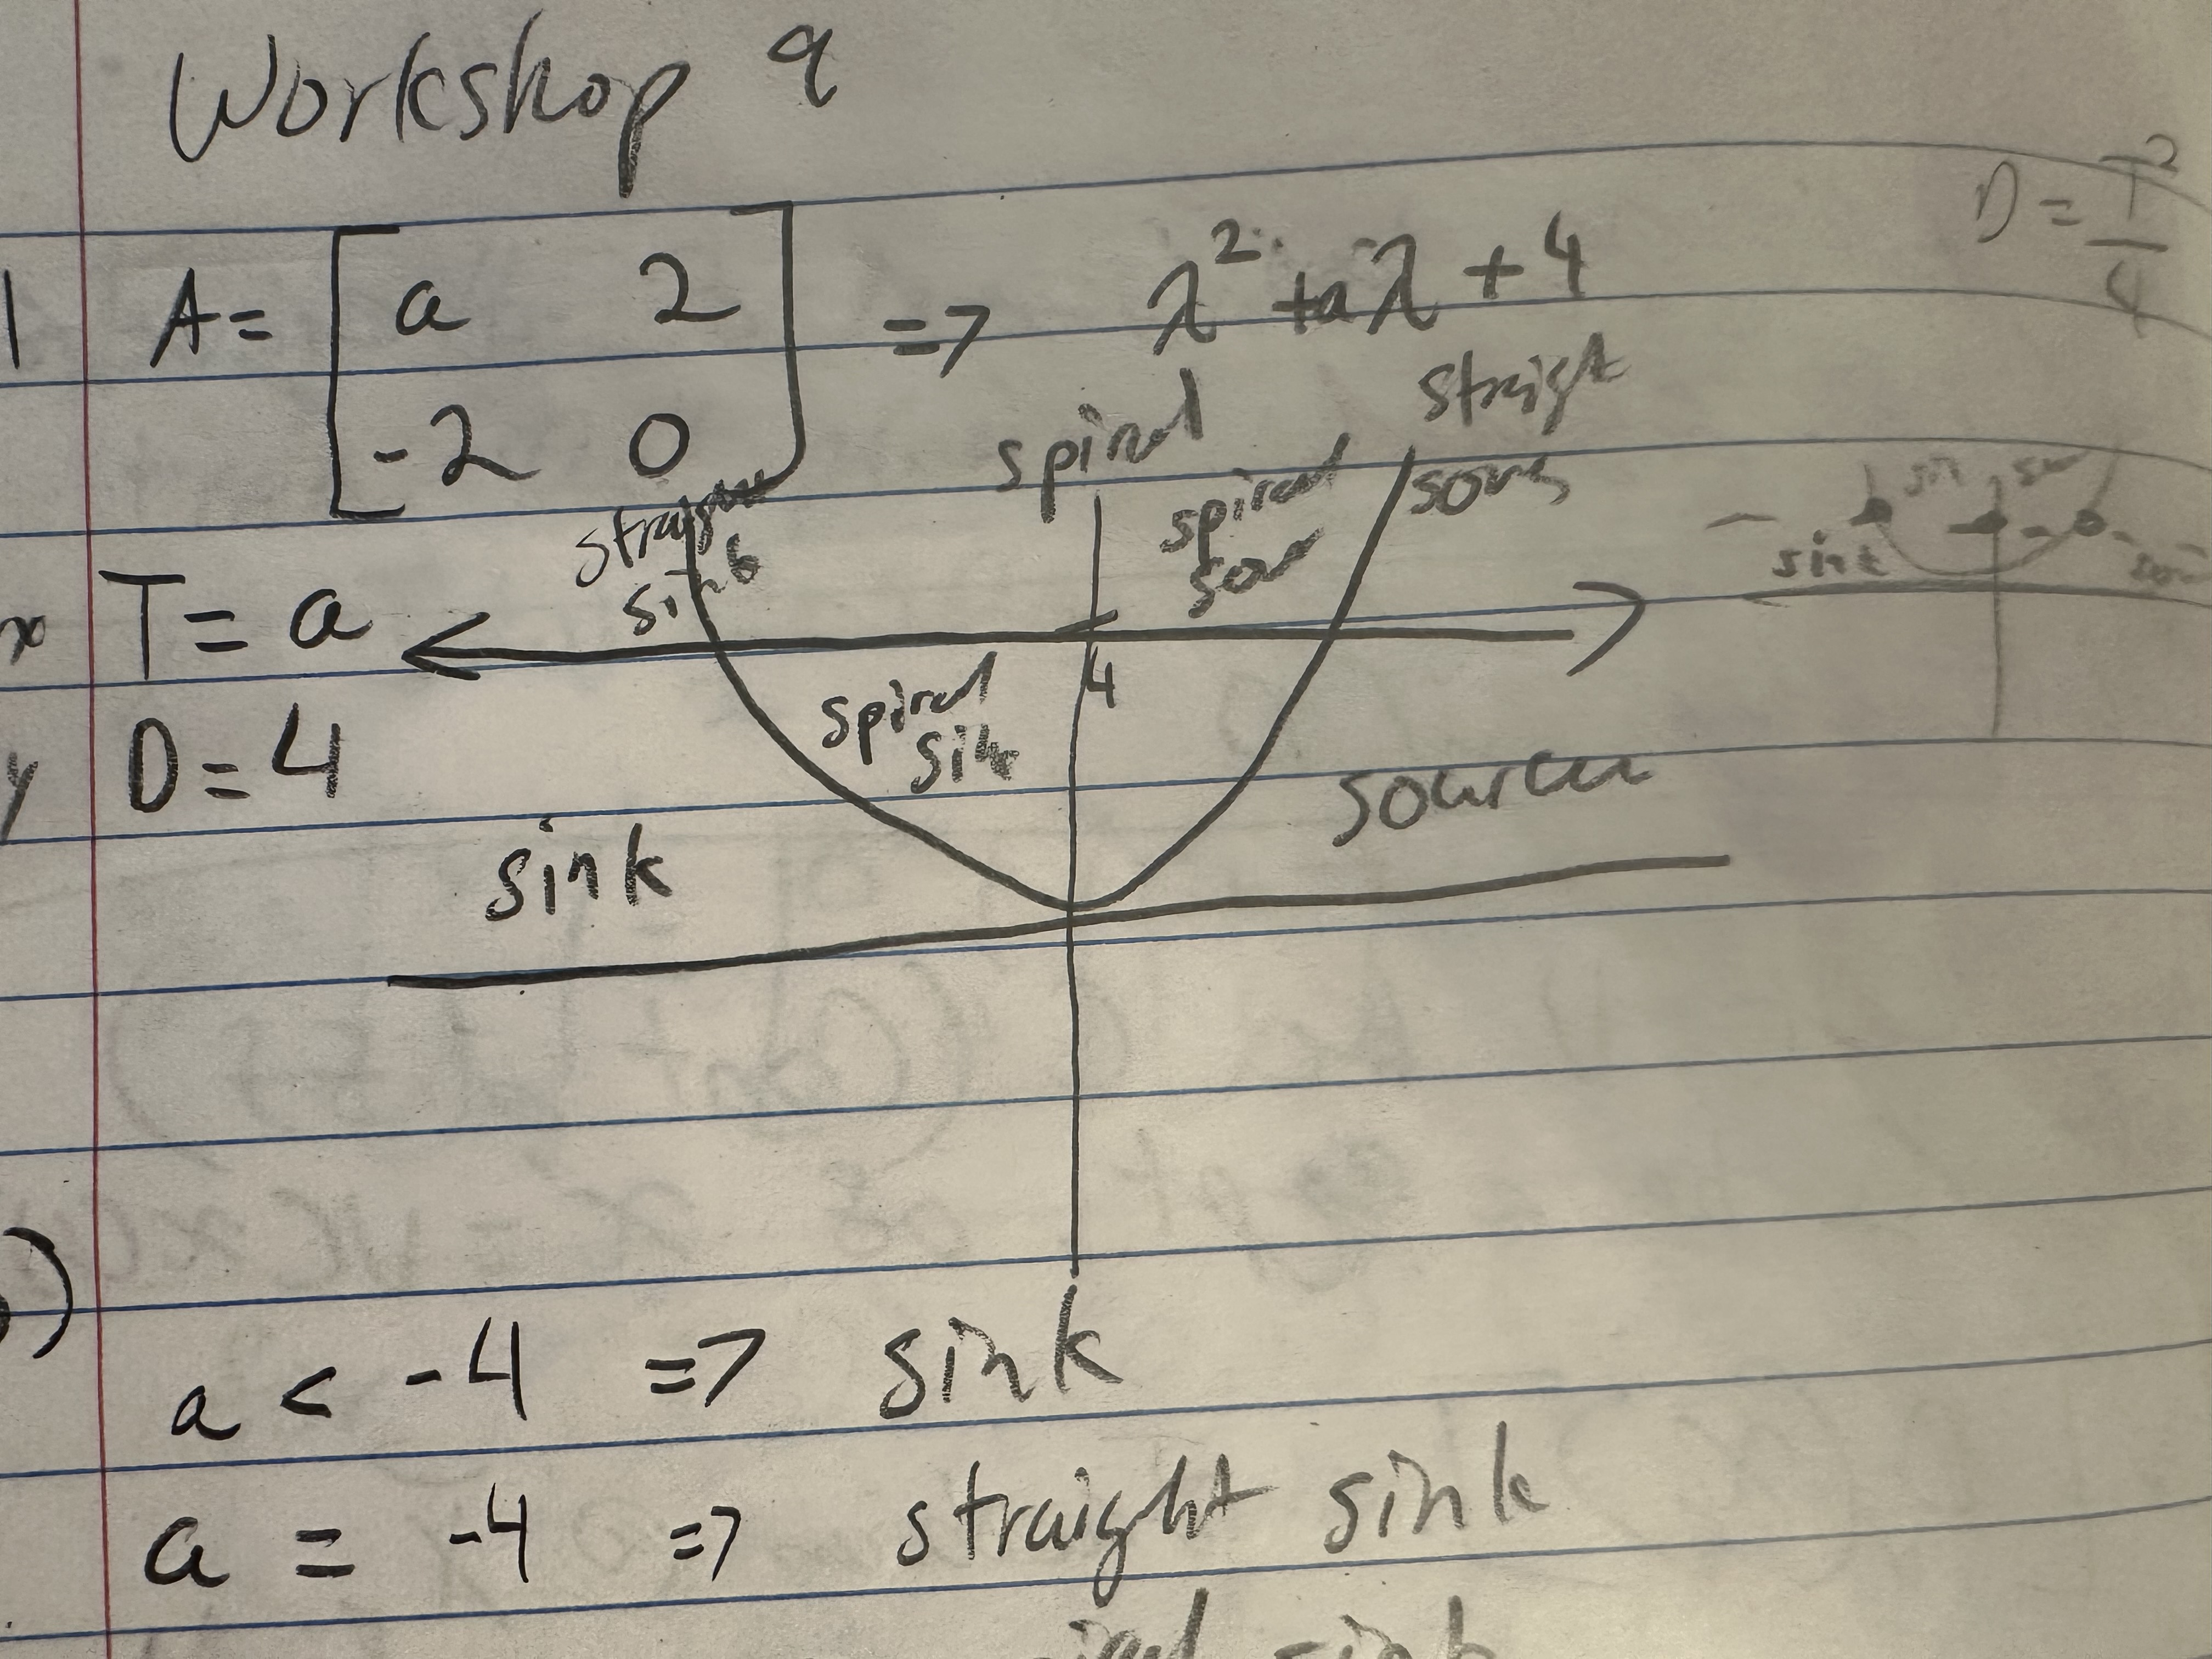
\includegraphics[width=0.5\textwidth]{IMG_2809.jpg}
\subsection*{b)}
Clearly the Line on the T-D graph has 7 distinct features:
\begin{enumerate}
    \item $a<-4$ sink
    \item $a=-4$ straight sink
    \item $-4<a<0$ spiral sink
    \item $a=0$ spiral 
    \item $0<a<4$ spiral source
    \item $a=4$ straight sources
    \item $a>4$ source 
\end{enumerate}
\section*{Question 2}
$x'(t) = x(1-(1/2)y)$ and $y'(t) = y(-3/4+(1/4)x)$
\subsection*{a)}
Equilibrum points: $(0,0)$ and $(3,2)$
\subsection*{b)}
The jacobian matrix is: $$\begin{bmatrix}
1-y/2 & -x/2\\
y/4 & -3/4+x/4
\end{bmatrix}$$
At $(0,0)$ the jacobian matrix is: $$\begin{bmatrix}
1 & 0\\
0 & -3/4
\end{bmatrix}$$
At $(3,2)$ the jacobian matrix is: $$\begin{bmatrix}
0 & -3/2\\
1/2 & 0
\end{bmatrix}$$
\subsection*{c)}
The eigenvalues at $(3,2)$ are $i\sqrt{3}/2,- i\sqrt{3}/2$. They have no real part
\subsection*{d)}
To prove the stability of the equilibrium points we need to observe that that the level curves of the system stay within a boundary. to do this we can solve for $\frac{dy}{dx}$ and find the level curves. 
$$\frac{dy}{dx} = \frac{y'}{x'} = \frac{y(-3/4+(1/4)x)}{x(1-(1/2)y)} $$
$$\int \frac{1-(1/2)y}{y}dy = \int \frac{-3/4+(1/4)x}{x}dx$$
$$\ln|y| - \frac{1}{2}y =  -\frac{3}{4}\ln|x| + \frac{1}{4}x + C$$
$$\ln|y| - \frac{1}{2}y +\frac{3}{4}\ln|x| - \frac{1}{4}x = C$$

\subsection*{e)}
By setting C to .023 we can see that $\epsilon$ is a boundary for the level curves.
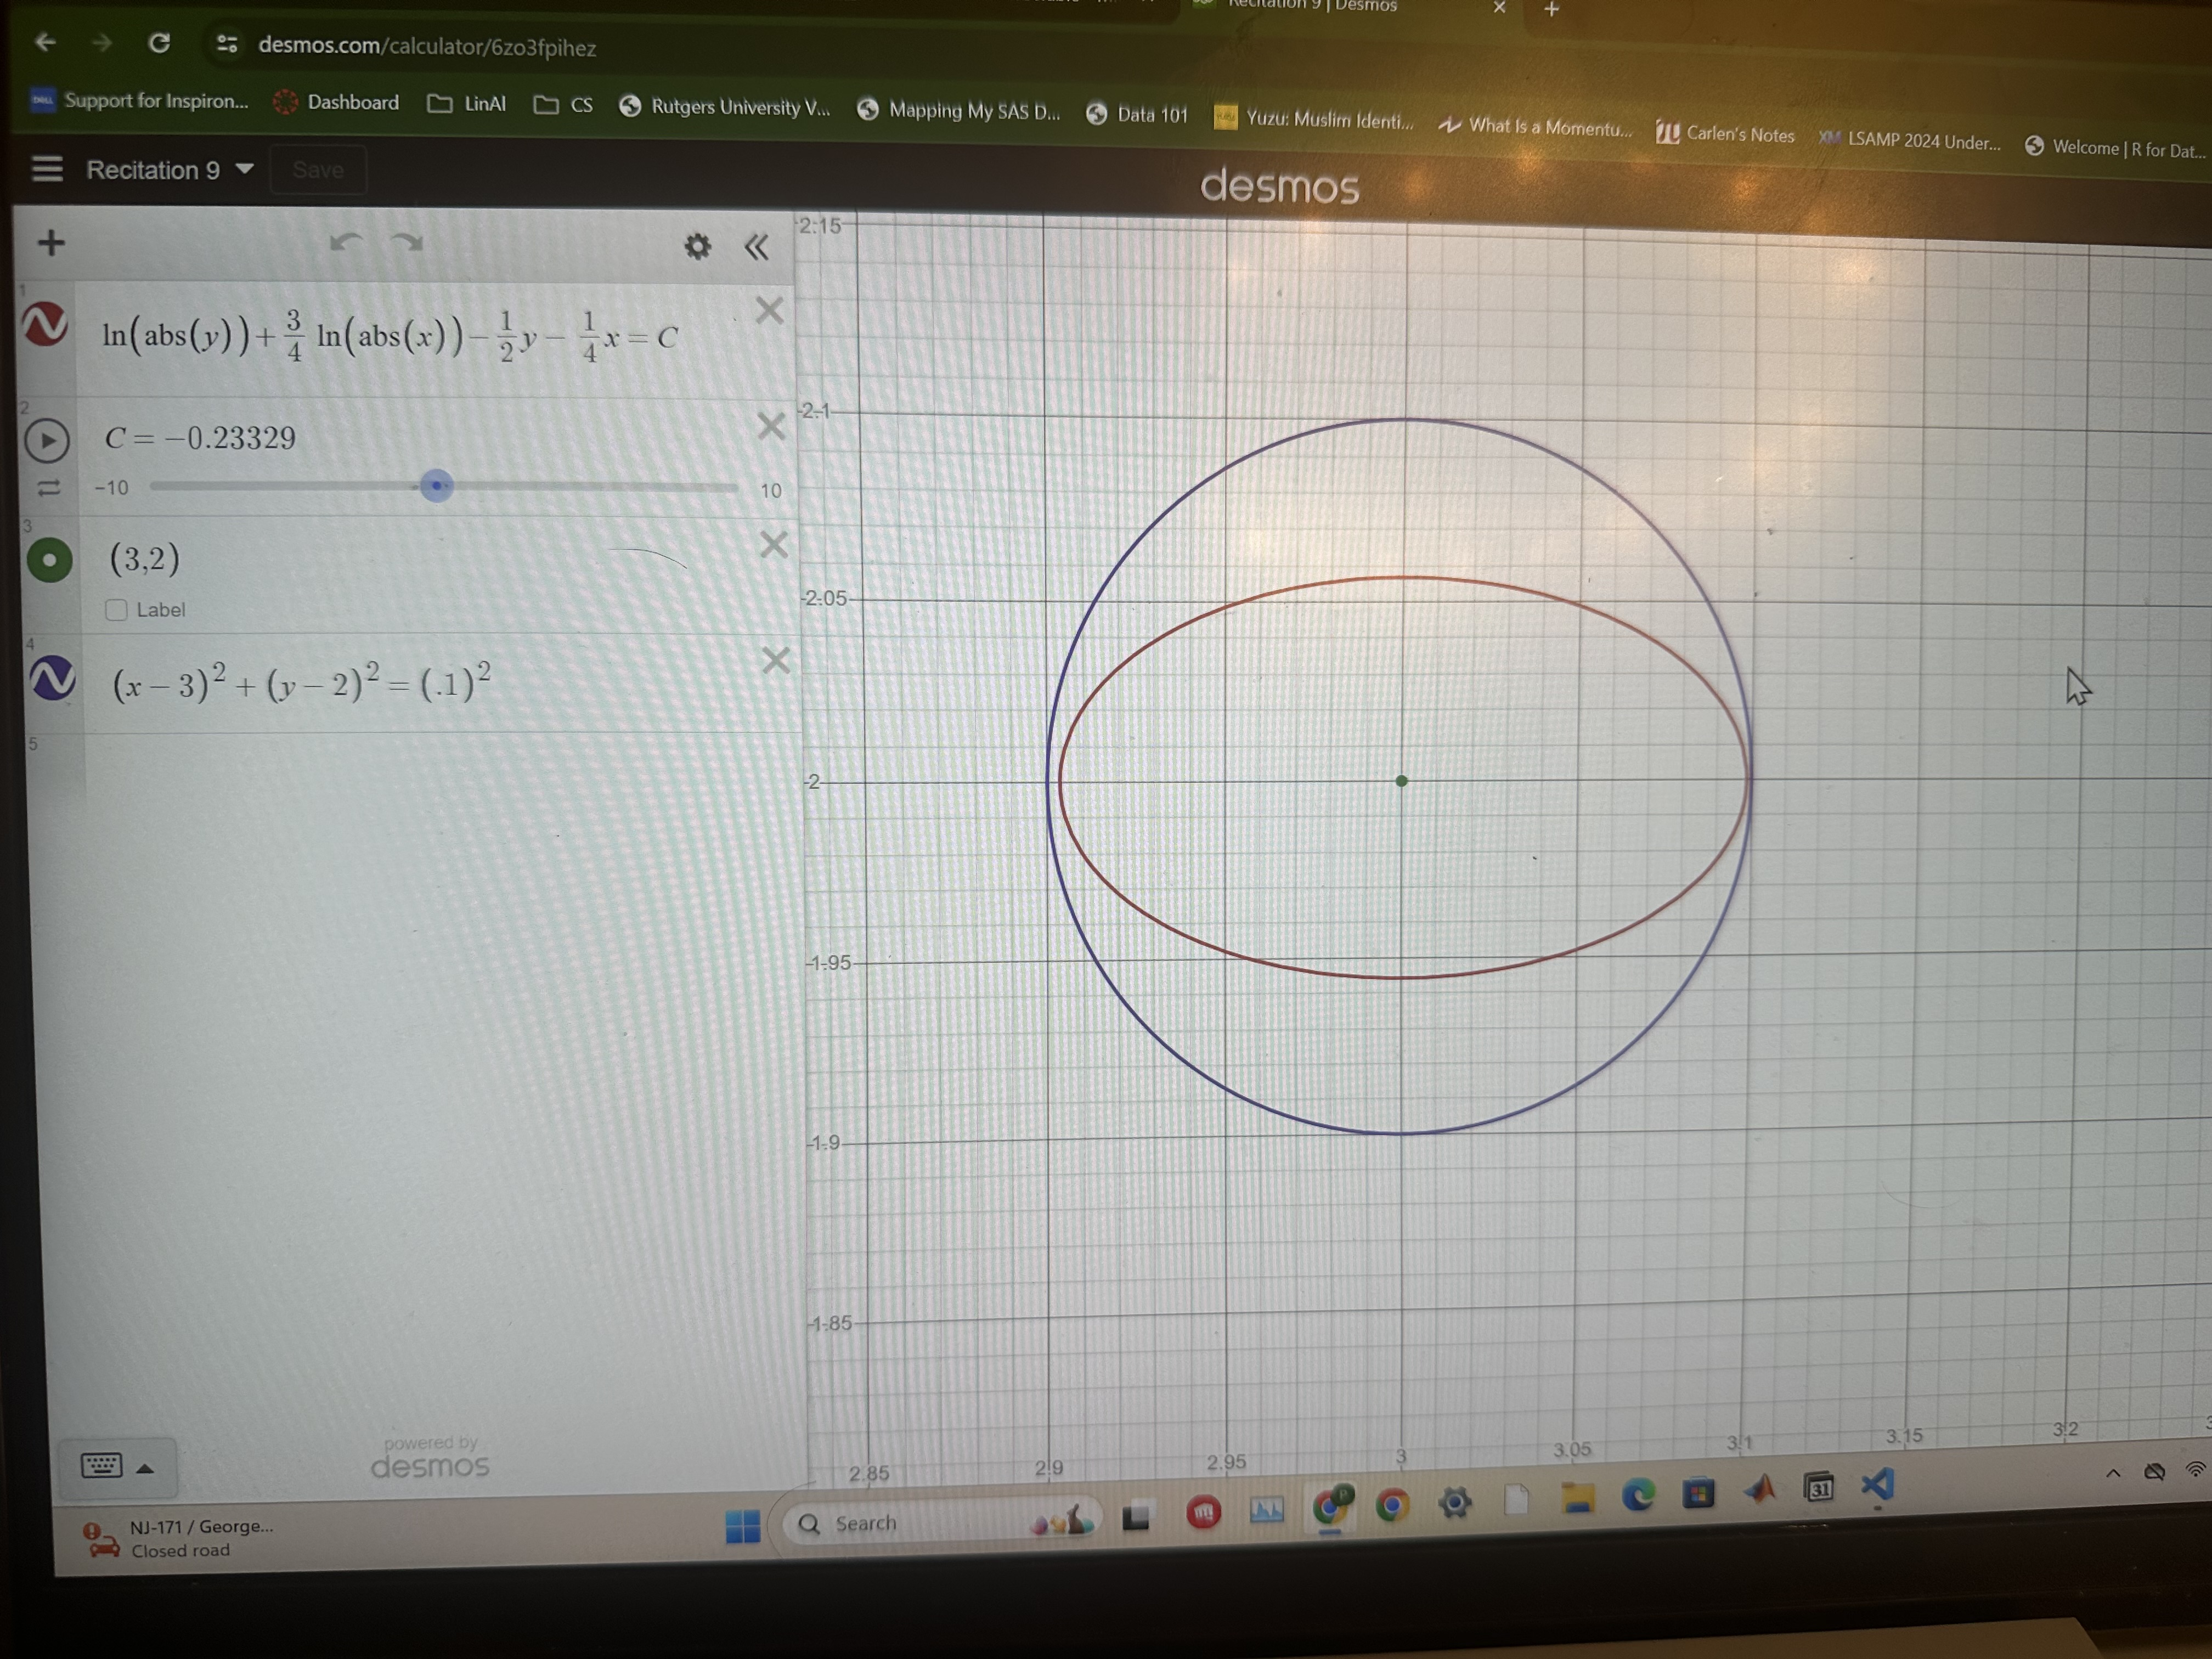
\includegraphics[width=0.5\textwidth]{IMG_2810.jpg}


\end{document}